\documentclass[a4paper,11.5pt,table]{article}
\usepackage[textwidth=170mm, textheight=230mm, inner=20mm, top=20mm, bottom=30mm]{geometry}
\usepackage[normalem]{ulem}
\usepackage[utf8]{inputenc}
\usepackage[T1]{fontenc}
\PassOptionsToPackage{defaults=hu-min}{magyar.ldf}
\usepackage[magyar]{babel}
\usepackage{amsmath, amsthm,amssymb, paralist, tikz, multirow}
\usetikzlibrary{arrows, positioning}

\usepackage{listings}
\lstset{
	language=C++, 
	basicstyle=\ttfamily, 
	keywordstyle=\color{blue}\ttfamily, 
	stringstyle=\color{red}\ttfamily,
	tabsize = 4
}

\usepackage{hyperref}

\begin{document}
	%%%%%%%%%%%RÖVIDÍTÉSEK%%%%%%%%%%
	\setlength\parindent{0pt}
	\def\<{<\hspace{0mm}<}
	
	\theoremstyle{definition}
	\newtheorem{note}{Megjegyzés}[subsection]
	%%%%%%%%%%%%%%%%%%%%%%%%%%%%%%%%%%%%%%%%%%%%%%%%%%%%%%%%%%%%%%%%%%%%%
	
	\begin{center}
		{\LARGE\textbf{C++}}
		
		{\Large Gyakorlat jegyzet}
		
		3 óra.
	\end{center}
	A jegyzetet \textsc{Umann} Kristóf készítette \textsc{Porkoláb} Zoltán és \textsc{Horváth} Gábor előadása alapján. (\today)
	%TODO Elkezdtem a még GSD által leadott kifejezések kiértékelését átírni, de megannyi óra szenvedés után is alig jutottam valahova, így egyenlőre kikommentezve hagyom.
%	\section{Kifejezések kiértékelése}
%	Ugorjunk vissza egy korábbi példára.
%	\begin{lstlisting}
%#include <iostream>
%
%int main()
%{
%	int i = 0;
%	std::cout << i << i++ << std::endl;
%}
%	\end{lstlisting}
%	%\< egy normálisabban kinéző << operátort eredményez (definíció fent)
%	
%	Világos, hogy a fenti kódban nem definiált viselkedés szerepel. Már volt szó arról is, hogy a kiíratáshoz használt \texttt{\<} szimbólum az egy operátor, és az \texttt{<iostream>} könyvtárban található hozzá egy olyan overload, melynek egyik paramétere \texttt{std::ostream\&}, a másik pedig \texttt{int}. Ahogy korábban is említve volt, az első paraméterével vissza is tér, így tudjuk a kiíratást láncolni. A fent leírt kiíratás ezzel lesz ekvivalens:
%	\begin{lstlisting}
%std::cout.operator<<(i).operator<<(i++);
%	\end{lstlisting}
%	
%	Itt látható egy \texttt{\<} operátor, ami így is felírható: \texttt{std::cout.operator$<<$(i)}. Ennek a függvényhívásnak van visszatérési értéke, méghozzá \texttt{std::cout}, így a függvényhívás láncolható. Ez itt egy member function, mellyel majdnem minden alaptípus  rendelkezik Ezalól kivétel a \texttt{std::string}, melynek \texttt{operator$>>$}-ja globális.
%	\begin{note}
%		Ennek az is lehet értelme, hogy ne függjön az operátor az osztálytól. Jó példa erre a \texttt{template}, mert annak csak akkor kell példányt létrehoznia, ha meghívják.
%	\end{note}
%	A fenti kódban lévő rész így is felírható:
%	
%	
%	Az, hogy a második szám 2 lesz, az biztos. De hogy az első mennyi, az nem definiált.
%	
%	\textit{1. ábra.}
%	
%	\begin{example}
%		\texttt{x = k + 2}\quad \quad \texttt{y = k + 2}
%	\end{example}
%	
%	Ebben a példában (jó eséllyel) a fordító kioptimalizálja ezt, és \texttt{k+2}-t csak egyszer számolja ki. A c++ban a nem szabványba foglalt szabályoknak köszönhetően sokkal hatékonyabb programokat kaphatunk, mert a fordítónak nagy szabadsága van abban, hogyan optimalizálja a kódunkat.
%	
%	\begin{example}
%		Itt a cél az lenne, hogy a tömb elemeit feltöltsük növekvő számokkal.
%		
%		\begin{lstlisting}
%int i = 0;
%int t[10];
%while (i < 10)
%{
%	t[i] = i++;
%}
%		\end{lstlisting}
%		
%		Azonban ez egy nem definiált viselkedés, mert hiába van ott egy \textbf{post-fix} \texttt{++}\quad operator, az hogy az egyenlőség melyik oldalán levő \texttt{i} értékelődik ki először, az ismét nem definiált.
%	\end{example}
%	
%	Itt leggyakrabban szekvenciapontok használata tud segíteni.
%	
%	\begin{definition}
%		(szekvenciapont) ami elválasztja, hogy mikor minek kell végrehajtódnia futási időben. A szekvenciapont előtt minden kifejezésnek ki kell értékelődnie. Több szekvenciapont létezik: vessző, \texttt{\&\&}, \texttt{||}, \texttt{?\quad :} 
%	\end{definition}
%	\begin{example}
%		\begin{lstlisting}
%f(i), ++i;
%i++<10 && f(i);
%i++<10 || f(i);
%i++<10 ? f(i) : g(i);
%		\end{lstlisting}
%		Ezek mint definiáltak, minden kifejezést egy szekvenkciapont választ el a másiktól.
%		\begin{lstlisting}
%f(i++, j++);
%		\end{lstlisting}
%		Itt azonban az, hogy i vagy j értéke növekszik-e meg először, az már nem definiált. Bár valóban található ott vessző, de a vessző mint szekvenciapont nem ekvivalens a függvény paramétereit elválasztó vesszővel.
%	\end{example}
%	\begin{note}
%		Az optimalizálás nagyon fontos szabálya, hogy mindig úgy szabad csak megtörténnie, hogy a program kimenetele ne változzon. 
%	\end{note}
%	\begin{note}
%		Ha hibásra optimalizálja a kódot a compiler, az nagy szívás. Ez leggyakrabban multi-threaded programoknál fordulhat elő.
%	\end{note}
%	
%	
%	\begin{lstlisting}
%int f() {cout << 'f'; return 2;}
%int g() {cout << 'g'; return 1;}
%int h() {cout << 'h'; return 0;}
%	\end{lstlisting}
%	Mi fog történni \texttt{f() == g() == h()} kód írásakor?
%	
%	Itt azon fog múlni a dolog, hogy milyen sorrendben értékelődnek ki az egyenlőség-vizsgáló operátorok. Az operátoroknak van megadott precedenciájuk: erős például a pont, nyíl, [], stb, gyengébb ennél a dereferencia, és így tovább. Azonban az azonos precedenciájú kifejezéseknél kérdéses, milyen sorrendben értékelődnek ki, vagy egyáltaln definiált-e az. Régen fortran-ban ez különösképp problémás volt:
%	
%	\begin{center}
%		\texttt{A*B / C*D}
%	\end{center}Itt nem lehetett tudni, hogy először megszorozza \texttt{A*B}-t, \texttt{D}-vel, és csak utána osztja le \texttt{C}-vel, vagy fordítva.
%	
%	Visszatérve a fenti példára, a végrehajtási sorrend:
%	\texttt{(f() == g()) == h()}. Azaz, a \texttt{==} operátor balről jobbra asszociatív. De milyen sorrendben lesznek kiírva a karakterek? Ez (brace yourselves) nem definiált., hisz az, hogy ezen belül melyik sorrendben fog kiértékelődni a függvényhívás, nincs meghatározva.
%	
%	Van ahol más a zárójelezés, pl. \texttt{!++*++p}. Itt Először előrelépünk a p pointerrel, dereferáljuk, megnöveljük az értékét, és negáljuk. \texttt{!(++(*(++p)))}. Ilyen példa szintén az egyenlőség operátor: \texttt{x = y = z = 3.14}. 
%	\begin{note}
%		Bővebben: \url{http://en.cppreference.com/w/cpp/language/operator_precedence}
%	\end{note}
%	Az optimalizációk azért is segítenek, mert platformspecifikusak gyakran. Úgy csinálja meg a fordítást, hogy az adott gépból a legtöbbet préselje ki.
%	%TODO sectiondivider
%	\begin{lstlisting}
%#include <iostream>
%
%char* answer (char *q);
%
%int main()
%{
%	std::cout << answer("Hogy vagy?") << answer("Biztos?") << std::endl;
%	return 0;
%}
%
%char* answer (char *q)
%{
%	std::cout << q;
%	static char buffer[80];
%	std::cin.getline(buffer,80);
%	return buffer;
%}
%	\end{lstlisting}
%	Itt már azt is meg akarjuk kérdezni, hogy biztos-e. Itt már találkoztunk a problémával, hogy a kiíratás sorrendje rossz. 
%	
%	\texttt{std::cout $<<$ answer("Biztos?") $<<$ answer("Hogy vagy?") $<<$ std::endl;}
%	
%	Ez már jó. (a kiértékelés nem definiált, de a kiíratási sorrend igen!)
%	
%	Ez az igazán jó megoldás, itt kevesebbet kell filózni:
%	
%	\text{std::cout $<<$ answer("Hogy vagy?");}
%	
%	\texttt{std::cout $<<$ answer("Biztos?");}
%	
%	Azonban a statikus változótól még nem szabadultunk meg. Egy másik megoldás lehet a dinamikus memória kezelés.
%	\medskip
%	
%	A dinamikusan lefoglalt memória az ,,átlagos'' stacken lévő objektumokkal szemben a mi felelőségünk teljesen. Nekünk kell őket allokálni, és ha nincs már rá szükségünk, nekünk is kell felszabadítani. c++11ben smart-pointerekkel ezt valamelyest automatizálhatjuk.
%	
%	\begin{lstlisting}
%#include <iostream>
%
%char* answer (char *q);
%
%int main()
%{
%	std::cout << answer("Hogy vagy?");
%	std::cout << answer("Biztos?");
%	return 0;
%}
%
%char* answer (char *q)
%{
%	std::cout << q;
%	char* buffer = new char[80];
%	std::cin.getline(buffer,80);
%	return buffer;
%}
%	\end{lstlisting}
%	Ez így nagyon szép megoldás, de a memória sajnos elúszott. Ahogy említve volt, a \texttt{new} kulcsszóval létrehoztunk a dinamikus tárhelyen egy új változót, de azt soha nem szabadítottuk fel. Ezért a legszebb megoldás még mindig az, hogyha referenciával átadok még egy paramétert, amiben el tudjuk tárolni a választ. Ennél azonban még egyszerűbb megoldás az, ha az \texttt{std::string}-et használjuk.
%	\begin{lstlisting}
%#include <iostream>
%
%std::string answer (char *q);
%
%int main()
%{
%	std::cout << answer("Hogy vagy?");
%	std::cout << answer("Biztos?");
%	return 0;
%}
%
%std::string answer (std::string q)
%{
%	std::cout << q;
%	std::string buffer;
%	std::cin >> buffer;
%	return buffer;
%}
%	\end{lstlisting}
%	
%	Ez a memóriában úgy néz ki, hogy a stacken létrejön egy pointer, heapre (vagy dinamikus tárhelyen) mutató területen tárolja el a buffert, copy konstruktorral adjuk vissza megoldást, a buffer destruktora felszabadítaná a tárhelyet. Ez így igen költséges. c++11ben annyi segítséget kapunk, hogy a move szemantika javít a hatékonyságon
	
	\section{Pointer aritmetika}
	\subsection{Konstans korrektség}
	Térjünk vissza a mutatókhoz. Volt már szó konstans mutatókról, ám konstans\textbf{ra} mutató mutatókról még nem.
	\begin{lstlisting}
const int ci = 6;
int *p = &ci;
	\end{lstlisting}
	A fenti kód nem fordul le, mert \texttt{ci} konstans, de \texttt{p} nem egy nem konstansra mutató pointer. Ez sértené a c++ban ismert \textbf{konstans korrektséget} (const correctness). A probléma az lenne, hogy ha fenti értékadás ehlyes lenne, akkor hiába lenne \texttt{ci} konstans, tudnánk módosítani \texttt{p}-n keresztül.
	\begin{lstlisting}
const int ci = 6;
const int *p = &ci;
	\end{lstlisting}
	Ez már jó lesz, mert a \texttt{p} egy konstansra mutató pointer, azaz tud mutatni olyan változókra, melyek konstansok. Egy konstansra mutató pointer \textbf{nem tudja megváltoztatni} a mutatott memóriacím értékét. Viszont egy konstansra mutató pointer még tud más memóriacímekre mutatni.
	\begin{lstlisting}
const int ci = 6;
const int *p = &ci;

int c = 5;
p = &c;
	\end{lstlisting}
	Ez is teljesen szabályos, konstansra mutató pointerrel nem konstans értékre mutathatunk. Ez azonban kellemetlen meglepetéseket is okozhat, hisz \texttt{c} nem konstans, azt továbbra is tudjuk módosítani (csak nem \texttt{p}-n keresztül)! Egy konstans pointer kezelése közben, mely által mutatott terület értékétől nem várnánk hogy változzon, gond nélkül módosulhat a mutatott érték.
	\begin{lstlisting}
const int *p = &ci;
int c = 5;
p = &c;
c = 5;
	\end{lstlisting}
	Szintaktikailag a *-ot sok helyre írhatjuk.
	\begin{lstlisting}
const int *p;
int const *p;
	\end{lstlisting}
	Egy kettő ugyanaz, mint fentebb láthattuk.
	\begin{lstlisting}
int * const p;
const int * const p;
int const * const p;
	\end{lstlisting} 
	Amennyiben a * után van a \texttt{const}, akkor egy \textbf{konstans pointert kapunk}, mely megváltoztathatja a mutatott értéket, de nem mutathat másra (konstans pointer \quad $\not=$\quad konstanra mutató pointer).
	\subsection{Mutatóra mutató mutatók} %lol
	Mutatóra mutató mutatók is léteznek, melyeket így tudunk definiálni:
	\begin{lstlisting}
int *p;
int **q = &p;
int ***r = &q;
	\end{lstlisting}
	Példaképp \texttt{q}-en keresztül meg tudjuk változni, \texttt{p} hova mutasson.
	\begin{lstlisting}
int c, d;
int *p = &c;
int **q = &p;
*q = &d;
	\end{lstlisting}
	Ezeket nagyon durván el lehet bonyolítani, ha konstans pointerekkel is dolgozunk, mellyel meg lehet akadályozni hogy egy pointeren keresztül ne lehessen módosítani hogy egy másik pointer hova mutasson.
	\begin{lstlisting}
int c, d;
int *p = &c;
int * const *q = &p;
*q = &d; // forditasi hiba
	\end{lstlisting}
	Mivel \texttt{q} egy \texttt{int}-re mutató konstans mutatóra mutató mutató, így csak egy olyan mutatóval tudunk rámutatni, ami egy \texttt{int}-re mutató konstans mutatóra mutató mutatóra mutató.
	\begin{lstlisting}
int c, d;
int *p = &c;
int * const *q = &p;
int *const ** const r = &q;
	\end{lstlisting}
	\begin{note}
		Megnyugtatás végett, mutatóra mutató mutató (**) még előfordul, de komplikáltabb ritkán.
	\end{note}
	\subsection{Függvény pointerek}
	C++ban lehetőségünk van arra is, hogy függvényeket adjunk át paraméternek.
	\begin{lstlisting}
int add(int a, int b)
{
	return a + b;
}

int mul(int a, int b)
{
	return a * b;
}

int reduce(int *start, int size, int initial, int (*op)(int, int))
{
	int ret = initial;
	for (int i = 0; i < size; i++)
	{
		ret = (*op)(ret, start[i]);
	}
	return ret;
}

int main()
{
	int t[] = {1,2,3,4,5};
	std::cout << reduce(t,5,0,&add) << std::endl;
	std::cout << reduce(t,5,0,&mul) << std::endl;
}
	\end{lstlisting}
	
	Itt \texttt{reduce} egy olyan paramétert is vár, mely igazából egy függvény, mely \texttt{int}-et ad vissza, és két \texttt{int}-et vár paraméterül.
	\begin{note}
		A szavakba öntés segíthet a megértésben: \texttt{op} egy olyan függvényre mutató mutató, melynek két \texttt{int} paramétere van, és \texttt{int} a visszatérési értéke.
	\end{note}
	
	A kódban feltűnhet, hogy a tömb mellé paraméterben elkértük annak méretét is. Ez azért van, mert a \texttt{t} tömb egy \texttt{int}-re mutató mutatóvá fog konvertálni, ami az első elemre mutat. Ennek hatására értelemszerűen elvesztjük azt az információt, hogy mekkora volt a tömb (a tömbök és paraméterátadás kapcsolátról később bévebben lesz szó). Így át kell adni ezt az információt is. 
	
	Mellékesen, függvényeket kezelni csak pointerekkel lehet, és mivel a fordító tudja hogy függvényeket akarunk átadni, a \texttt{\&} jel elhagyható függvényhíváskor, és az \texttt{op} elől is elhagyható a * a paramétereknél.
	\begin{lstlisting}
int reduce(int *start, int size, int initial, int op(int, int)))
{
	//...
}

int main()
{
	int t[] = {1,2,3,4,5};
	std::cout << reduce(t,5,0,add) << std::endl;
	std::cout << reduce(t,5,0,mul) << std::endl;
}
	\end{lstlisting}
	\section{Tömbök}
	A tömbök a c++ alapértelmezett konténere, mellyel egyszerre tömb azonos típusú elemet kezelhetünk. Előzménytárgyakból már megismertük valamennyi funkcionalitását, ám számos veszélyét még nem.
		\begin{lstlisting}
int main()
{
	int i = 5;
	int t[] = {5,4,3,2,1};
}
		\end{lstlisting}
		\texttt{t} egy 5 elemű \textbf{tömb}. Nézzük meg, mekkora a mérete (figyelem, ez \textbf{implementációfüggő!})!
		\begin{lstlisting}
std::cout << sizeof(i) << std::endl;
std::cout << sizeof(t) << std::endl;
		\end{lstlisting}
		A \texttt{sizeof} operátor megadja a paraméterként megadott típus, vagy objektum esetében annak típusának méretét (bővebben később). Ez minden implementációra specifikus. Azt látjuk, hogy mindig ötszöröse lesz a \texttt{t} az \texttt{i}-nek. Azaz a tömbök tiszta adatok.  Stacken ábrázolja így képzeljük el:
		
		\begin{figure}[!h]
			\centering
			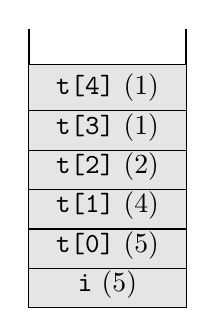
\begin{tikzpicture}
				\tikzstyle{Node} = [rectangle, minimum width=2cm, minimum height=5mm, text centered, draw=black, fill= gray!20]
				\tikzstyle{arrow} = [thick,->,>=stealth]
				
				\draw [thick, black] (0, 0) -- (2, 0);
				\draw [thick, black] (0, 0) -- (0, 3.5);
				\draw [thick, black] (2, 0) -- (2, 3.5);
				\node (c2) [Node] at (1,0.25) {\texttt{i} (5)};
				\node (d2) [Node] at (1,0.75) {\texttt{t[0]} (5)};
				\node (d2) [Node] at (1,1.25) {\texttt{t[1]} (4)};
				\node (d2) [Node] at (1,1.75) {\texttt{t[2]} (2)};
				\node (d2) [Node] at (1,2.25) {\texttt{t[3]} (1)};
				\node (d2) [Node] at (1,2.75) {\texttt{t[4]} (1)};
			\end{tikzpicture}
			\smallskip
			
			A \texttt{main} függvény változói.
		\end{figure}
		\subsection{Biztonsági rések nem definiált viselkedés következében}
		Irassuk ki a a tömb elemeit! (de ezt basszuk is el!)
		\begin{lstlisting}
for (int i = 0; i < 6; i++) //nem 6 elemes
{
	std::cout << t[i] << std::endl;
}
		\end{lstlisting} 
		Itt előre látható, hogy túl fogunk indexelni. Ez így egy {nem definiált viselkedés}hez vezet. Várhatóan valamilyen random memóriaszemetet fog kiolvasni (vagy olvashat ki, lévén nem definiált), és sose tudhatjuk pontosan mit.
		
		Most növeljük meg az elemeket, és menjünk el egészen 100ig!
		\begin{lstlisting}
for (int i = 0; i < 100; i++)
{
	++t[i];
}
std::cout << "sajt" << std::endl;
		\end{lstlisting} 
		Ez szintén nem definiált. Mivel olyan memóriaterületeket szeretnénk módosítani, melyeket nem foglaltunk le a programunknak, bajba juthatunk. Itt az órán a {sajt} szöveg ki lehet írva, mégis kaptunk szegmentálási hiba (\textit{segmentation fault}) hibaüzenetet az oprendszertől.
		
		\begin{lstlisting}
for (int i = 0; i < 100000; i++)
{
	++t[i];
}
std::cout << "sajt" << std::endl;
		\end{lstlisting} 
		Itt már (legalábbis ebben az esetben) előbb vágta magát hanyat a program, mielőtt sajt-ot ki tudta volna íratni. Ez jól demonstrálja, hogy ugyanazt  a hibát követtük el, de más volt a végeredmény. Ezért igazán veszélyesek a nem definiált viselkedések.
		\begin{lstlisting}
#include <iostream>
#include <string>

int main()
{
	int t[] = {5,4,3,2,1};
	int isAdmin = 0;
	std:string name;
	std::cin >> name;
	for (int i = 0; i < name.size(); ++i)
	{
		t[i] = 1;
	}
	if (name == "pityu")
		isAdmin = 1;
	std::cout << "Admin?: " << (isAdmin != 0 ) << std::endl;
}
		\end{lstlisting}
		Ha a programnak \texttt{pityu}-t adunk meg amikor be akarja olvasni \texttt{name}-et, akkor minden a legnagyobb rendben. De mivel a forráskódot ismerjük, azért hogyha nagyon hosszú nevet adnánk (nagyobb mint 5), akkor a túlindexelés miatt ki tudjuk használni a nem definiált viselkedéseket, és az is előfordulhat, hogy az \texttt{isAdmin} memóriacímére írunk, és elérjük hogy akkor is adminnak higgyen minket, ha nem vagyunk azok.
		\medskip
		
		Hogyan lehet ezeket a hibákat elkerülni? Túl azon, hogy nagyon figyelni kell, vannak programok amik segítenek nekünk. Ehhez használhatunk \texttt{sanitizer}-eket. Ezek picit módosítanak a kódunkon, és amennyiben futási időben bizonyos nem definiált viselkedéseket követne el, pl. itt a túlindexelés, leütné a programunkat. Használatukhoz elég egy extra paranccsal fordítanunk:
		
		{\centering\texttt{g++ main.cpp -fsanitize=address}\par }
		
		De sajnos ez is csak akkor tud segíteni, ha a probléma előfordul (azaz futási időben, nem fordítási időben ellenőriz). Amennyiben előfordul viszont, elég pontos leírást tudunk kapni arról, hogy merre van a probléma.
		
		{\centering \texttt{g++ main.cpp -Wall -Wextra} \par}
		
		Ez a 2 parancs szintén extra ellenőrzéseket vezet be, de nem változtatják meg a kódot, csak fordítási időben ellenőriznek.
	\subsection{Hivatkozás tömb elemeire}
		\begin{lstlisting}
#include <iostream>

int main()
{
	int t[] = {5,4,3,2,1};
	int *p = t;
	std::cout << *p << std::endl;
	std::cout << sizeof(int) << std::endl;
	std::cout << sizeof(p) << std::endl;
	std::cout << sizeof(t) << std::endl;
}
		\end{lstlisting}
		Könnyű azt hinni (hibásan) hogy a pointerek ugyanazok mint a tömbök. Ez  program jól mutatja, hogy ez nem igaz, mert a tömb tárolja annak méretét is. Számos más különbség is van, viszont egy tömb könnyen konvertálódik pointerré.
		
		Egy tömb adott elemét sokféleképpen le tudjuk kérdezni:
		
		{\centering \texttt{*(p + 3) == *(3 + p) == p[3] == 3[p]} \par}
		\
		\begin{lstlisting}
#include <iostream>

int main()
{
	int t[][3] = {{1,2,3},{4,5,6}};
	return 0;
}
		\end{lstlisting}
		Ez egy alternatív módja egy tömb inicializálásának. Itt több dolog megfigyelendő: Az első \texttt{[]} operátorban nincs méret, mert a fordító az inicializáció alapján meg tudja állapítani, hogy a mátrix azon dimenziója mekkora, de annyira már nem okos, hogy a másodikat is abszolválja.
		
		\medskip
		Fontos megjegyezni, hogy a mátrix egy adott elemére még többféleképpen tudunk hivatkozni:
		\medskip
		
		\begin{center}
			\texttt{t[1][] == *(*(t+1)+0) == *(1[t]+0) == 0[1[t]] == 0[*(t+1)] == *(t+1)[0] == 1[t][0] } 
		\end{center}
	\begin{note}
		Ahhoz, hogy egy olyan függvényt írjunk ami minden méretű tömböt elfogad paraméterül, a legegyszerűbb megoldás, ha hagyjuk, hogy a tömb átkonvertáljon egy olyan pointerré, ami az első elemre mutat, és átadjuk külön paraméterben a tömb méretét. Bár van megoldás arra is, hogy egy darab "rugalmas" függvényt írjunk, és az egész tömbhöz csak 1 paramétert vegyünk át, annak is komoly hátulütői lehetnek. Majd template-ekkel a 7-8. gyakorlaton lesz részletesen szó, de kb így nézne ki:
		\begin{lstlisting}
template <class T, int ArraySize>
void ( T (&param)[ArraySize] )
{
	//...
}
		\end{lstlisting}
		\smallskip
		Ez később jobban ki lesz fejtve, de itt egy template paraméter dedukció fog létrejönni, és a fordító kitalálja \texttt{param} méretét. Csak nyilván, mindig amikor egy más méretű tömböt hozunk létre, a fordító példányosítja ezt a függvényt, ami csúnyán meg tudja dobni a bináris kódot (\textit{binary code}).
		
		\smallskip
		A tömbök átvétele paraméterként azért ilyen körülményes, mert egy tömbnek a méretét fordítási időben ismernünk kell. Ha változó méretű tömböt várnánk paraméterül, az szembemenne ezzel a követelménnyel.  
	\end{note}
	\begin{note}
		Progalapon úgy tanultunk tömböket, hogy változó méretet adtunk meg nekik. Ezt a \texttt{gcc} compiler elfogadja, lefordítja, és jó kódot is csinál belőle, de nem garantált, hogy ezt minden fordító megteszi, ugyanis a c++ szabvány azt mondja ki, hogy a tömb méretének fordítási időben ismertnek kell lennie. Ez jól demonstrálja, hogy a compilerek nem feltételnül követik szorosan a szabványt.
	\end{note}
\end{document}
